\subsection{Général}
	Le fait de développer des applications \gls{ios} et \gls{android}, nous a 
	imposé le choix du langage.
	En effet pour développer des applications \gls{iphone}, il faut utiliser 
	le langage \gls{objective-c}.
	Pour les applications \gls{android} c'est le langage \gls{java} qui est 
	utilisé.
	
	Ces deux langages ont une syntaxe complétement différente mais sont quand 
	même très proches car ce sont des langages orientés objets.
	Grâce à cela nous avons pu mettre au point une modélisation générale de 
	l'application que nous avons ensuite adapté à chaque langage.\\
			
	Nous avons décidé de développer en anglais car premièrement c'est la langue
	la plus utilisée dans le monde de la programmation et deuxièmement car la 
	syntaxe des langages est toujours en anglais.
	Cela permettra à n'importe quel utilisateur de n'importe quelle nationalité 
	de comprendre le code de l'application.\\
			
	La documentation des deux applications est également en anglais.
	Cette documentation permettra à tout utilisateur de comprendre le 
	fonctionnement de celle-ci, que ce soit sur \gls{iphone} ou \gls{android}.
	
	Chacune d'elles est au format \gls{html} et sera donc directement visible 
	grâce à un navigateur Web.\\
			
	Pour ce qui est de la modélisation globale du projet, nous avons choisi de 
	développer les deux applications selon le modèle \gls{mvc}.
	Ce dernier est une architecture et une méthode de conception qui organise 
	l'\gls{ihm} d'une application logicielle. 
			
	Le modèle représente le comportement de l'application : traitements des
	 données, interactions avec la base de données, etc.
	Il décrit et contient les données manipulées par l'application, assure 
	la gestion de ces données et garantit leur intégrité.
			
	La vue correspond à l'interface avec laquelle l'utilisateur interagit.
	Sa première tâche est de présenter les résultats renvoyés par le modèle.
	La seconde est de recevoir toutes les actions de l'utilisateur 
	(clic de souris, sélection d'une entrée, boutons, etc).
			
	Le contrôleur prend en charge la gestion des événements de synchronisation 
	pour mettre à jour la vue ou le modèle et les synchroniser.
	Il reçoit tous les événements de l'utilisateur et enclenche les actions 
	à effectuer.
			
	Grâce à cette méthode de conception le code est décomposé en trois parties 
	bien distinctes qui permettent la maintenance et l'amélioration du projet.
	Cela permet aussi d'améliorer chacune des trois parties sans avoir à 
	modifier les deux autres.
	Par exemple de changer de vue et donc avoir des interfaces graphiques différentes.
			
\subsection{Menus}

	Au démarrage de l'application vous arrivez sur un menu d'accueil. Depuis
	celui-ci vous pourrez accéder à l'aide, à la liste des comptes locaux ou à la
	création d'un nouveau compte local.
	
	Ils se divisent en quatre grandes sections.
		
	Premièrement la section de création de parties locales dans laquelle l'utilisateur
	pourra choisir parmit une liste de cartes celle sur laquelle il désire jouer.
	Le réglage de la difficulté des \glspl{bot}, leur nombre et le temps de jeu.
		
	Dans la même catégorie se trouve la section des parties multijoueurs. En
	accédant à celle-ci vous allez pouvoir vous connecter à votre compte
	multijoueur ou le créer s'il n'est pas déjà fait. Vous accèderez ensuite à la liste
	des parties multijoueurs, que vous pourrez rejoindre ou choisir de créer la
	votre. Dans le menu création le principe est proche des parties locales.
		
	Suite à ces deux sections vient ensuite l'éditeur de cartes.
	C'est depuis ce menu que vous créerez une nouvelle map de jeu local ou 
	éditerez l'une d'entre elles.
		
	Enfin vient le menu des options où vous pourrez gérer vos
	préférences sytèmes telles que le volume ou la langue de
	l'application(anglais, français).
	Une sous-section de gestionnaire de profil est aussi présente.
	Une édition de vos comptes locaux, multijoueurs ou même
	vos paramètres de jeu comme la position du menu, sont modifiable depuis ce 
	menu.
	
	\begin{figure}
		\label{activité}
		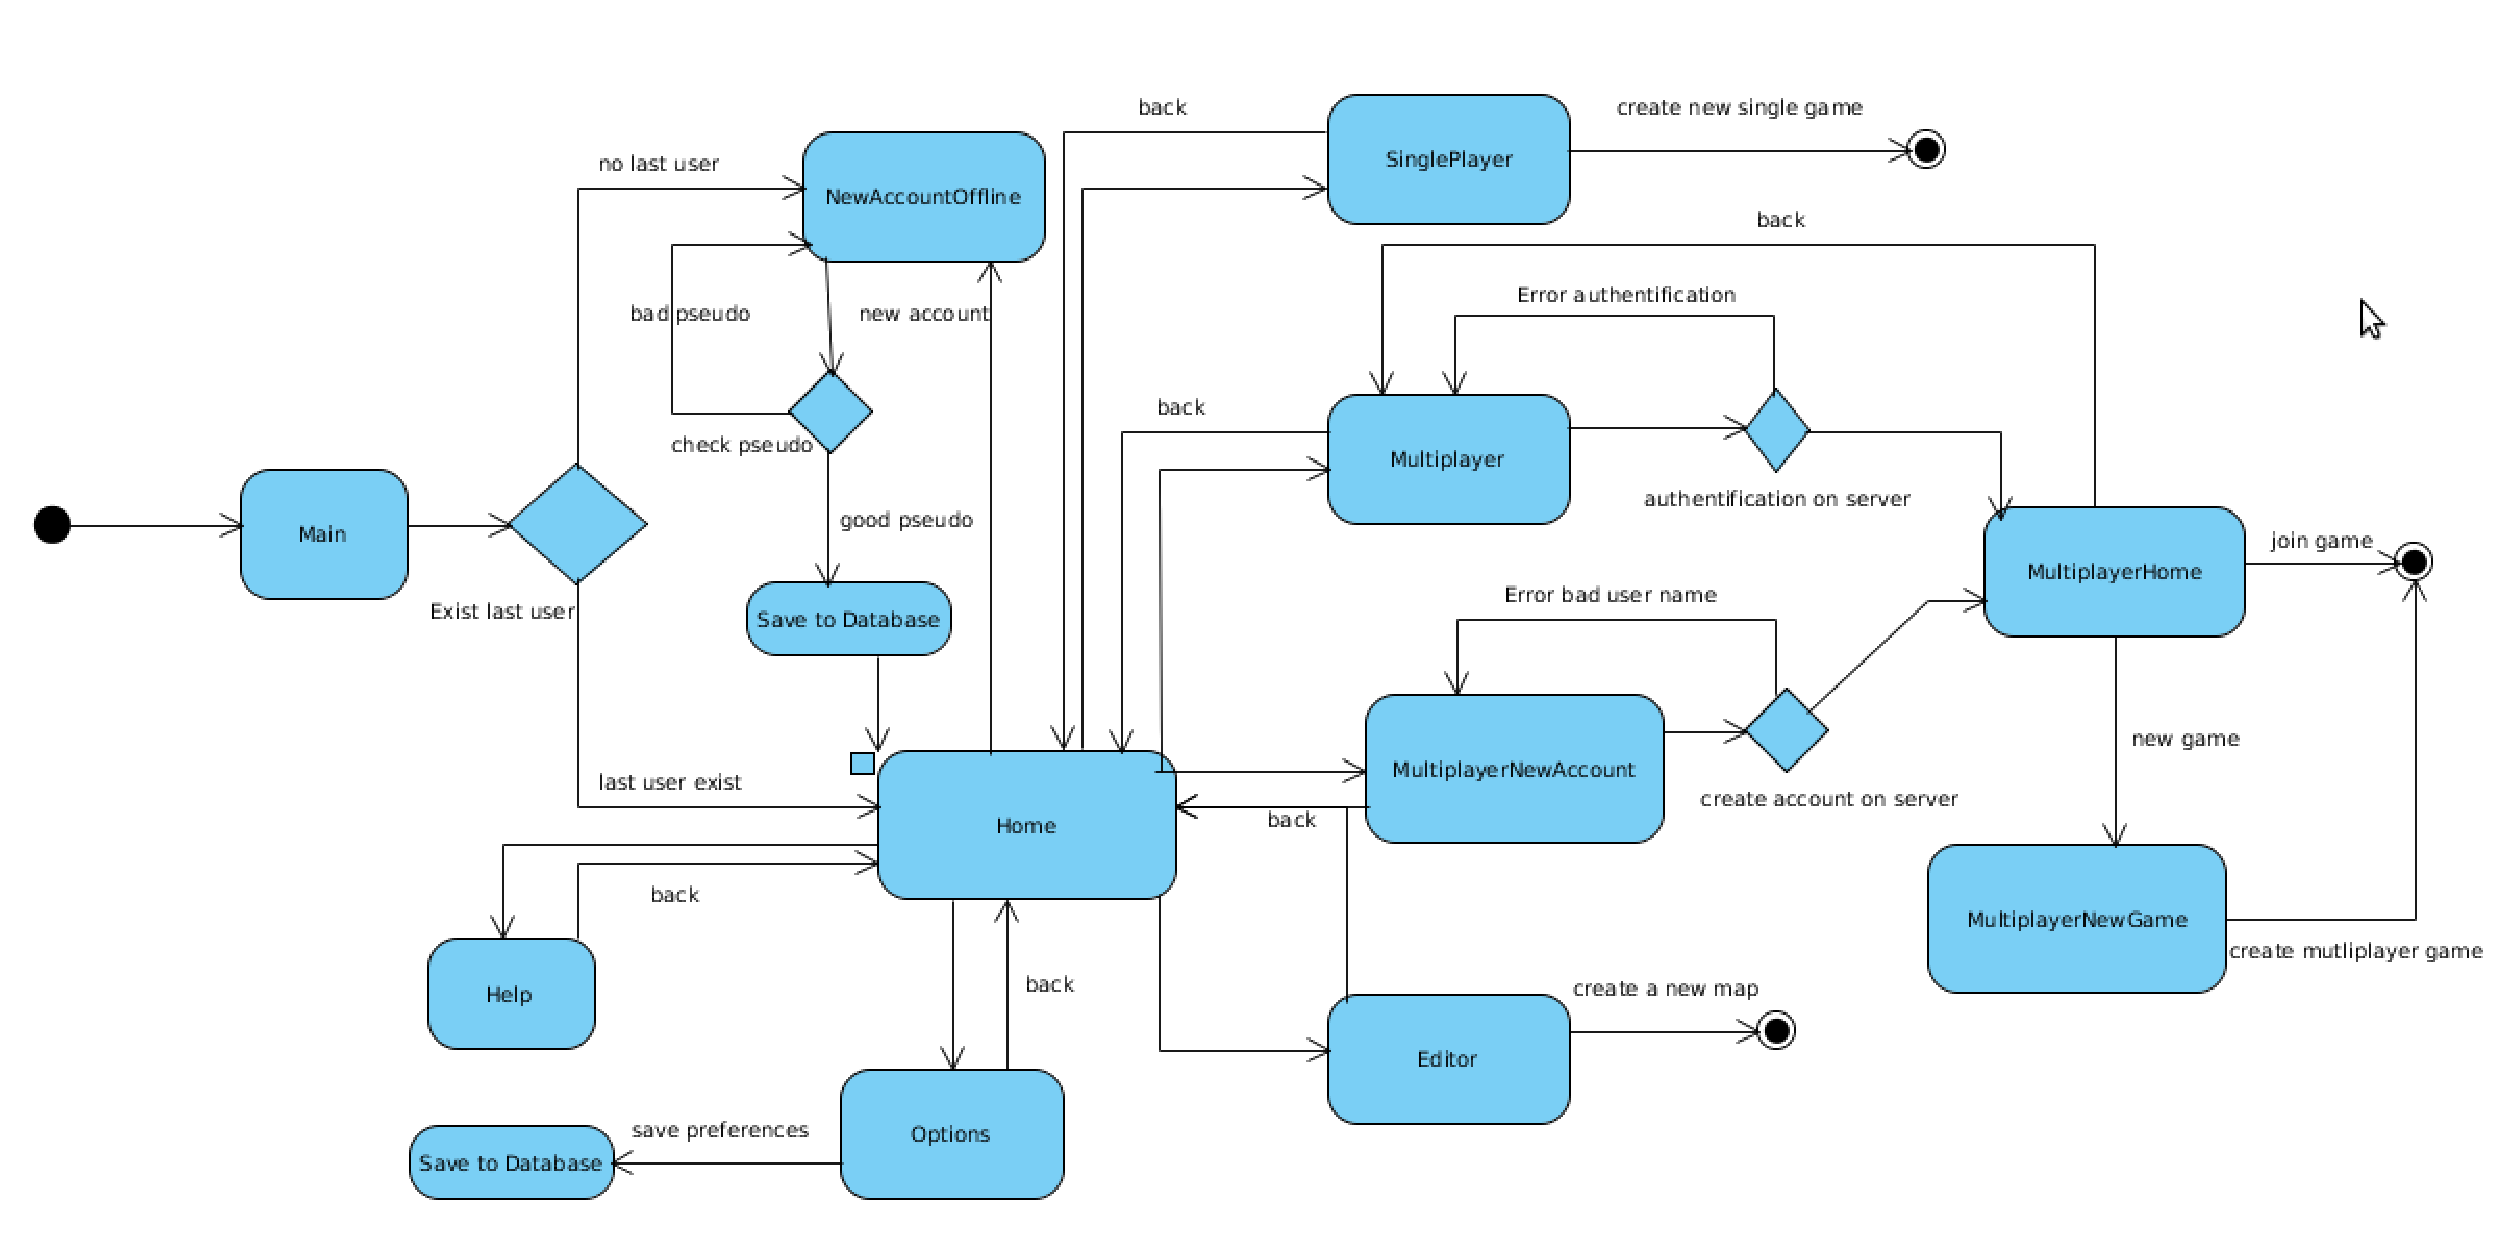
\includegraphics[width=23cm, angle=90]{Analyse/Img/diag_activity.eps}
		\caption{Diagramme d'activité}
	\end{figure}

	\paragraph{Base de données\\}
			
		Une base de données locale a elle aussi été conçue. Cette dernière a pour
		but de stocker plusieurs types de données.
				
		En effet dès lors qu'un compte local est créé sur le téléphone dans la
		table PlayerAccount, il est possible de conserver ses préférences telles 
		que la couleur du joueur, le pseudonyme ou même ses paramètres de connexion multijoueur.
				
		L'application est par ailleurs en mesure de conserver
		les valeurs sonores, la langue et même le dernier utilisateur de
		l'application grâce à un son identifiant qui est clé étrangère dans la table System(attribut lastUser).
				
		De plus l'application sera délivrée avec quelques cartes officielles, mais
		l'utilisateur aura libre droit de créer ses propres cartes de jeu via un
		éditeur. Elles seront alors stockées dans la table Map avec toujours une
		clé étrangère vers l'identifiant de son créateur. \\
		
		\newpage
				
		\begin{figure}
			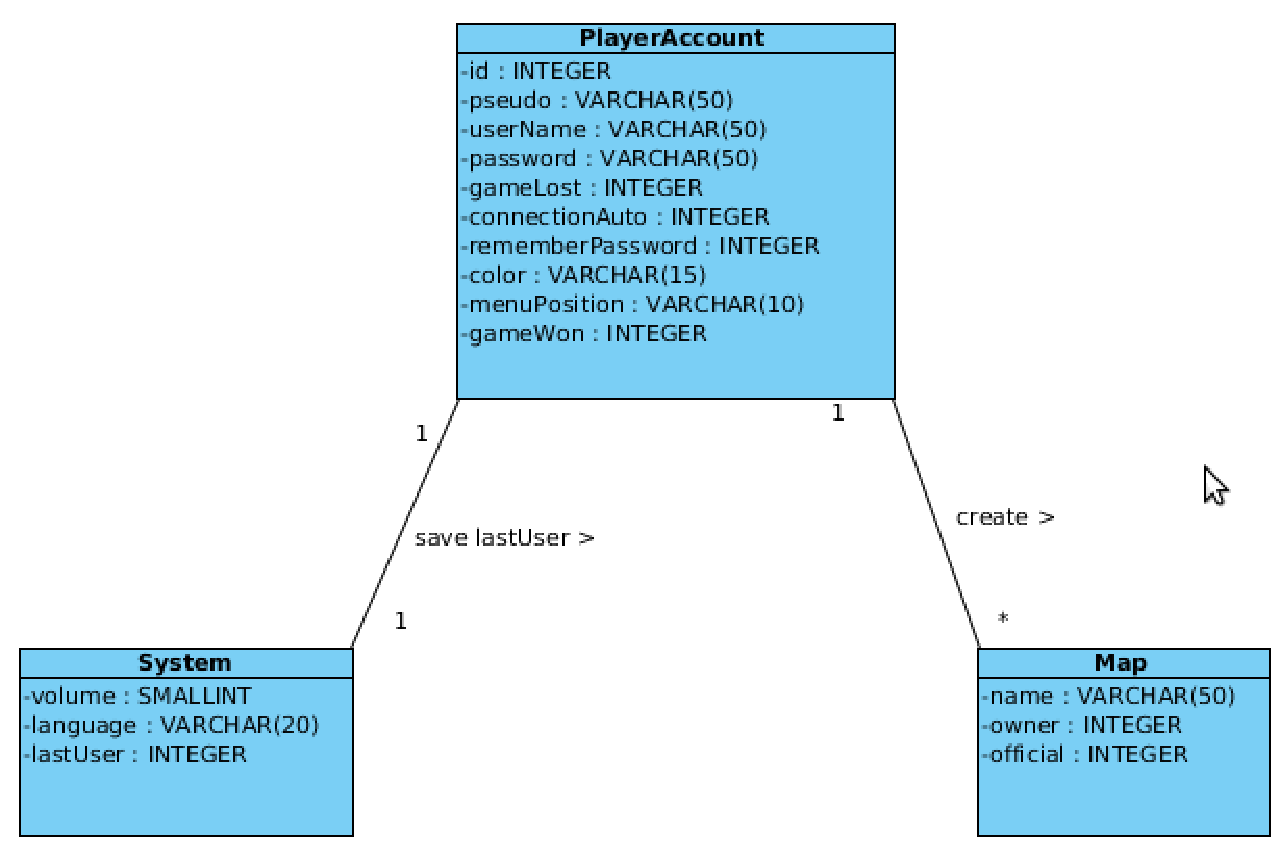
\includegraphics[width=11cm]{./Analyse/Img/menu_bdd.eps}
			\caption{Diagramme de classe Base de données}
		\end{figure}	
	
\subsection{Editeur de carte}	

	L'éditeur de carte est une fonctionnalité qui va permettre à un utilisateur
	 de créer facilement ses propres cartes pour ensuite y jouer dessus contre 
	 l'intelligence artificielle.
	 
	Après avoir réfléchi sur toutes les fonctionnalités que l'éditeur de carte 
	devait remplir, nous avons retenu celles-ci : permettre à l'utilisateur de 
	d'en créer une nouvelle, mais aussi de pouvoir charger une ancienne carte 
	précèdemment créée.
	
	Il peut de modifier le sol de la carte, ajouter ou supprimer des blocs de 
	la carte et enfin placer les différents points de départ des joueurs sur 
	la carte.
		
	Pour réaliser cette partie de l'application, nous avons aussi utilisé le 
	modèle de conception MVC.

	\subsubsection*{Modèle}
		La partie modèle va contenir toute les données de l'éditeur de carte. Les cartes sont les principales données qu'il va devoir manipuler. Pour cela nous avons décidé de la réprésenter sous la forme de deux matrices, la première représentant les objets du premier niveau (le sol) et la deusième la matrice du second niveau (les blocs, les points de départ des joueurs, etc).
			
			
	\subsubsection*{Vue}
		Ensuite, la vue représentera l'interface graphique de notre éditeur de carte. La principale difficulté pour réaliser l'interface graphique était de devoir rentrer toutes les informations nécessaires pour l'éditeur de carte dans un écran de type \gls{smartphone}. Après plusieurs prototypes d'interface, nous avons décide de séparer l'interface en trois parties. Tout d'abord la plus grande partie, l'affichage de la carte, qui comment étant la principale information à afficher, nous avons essayé de maximiser sa taille. Ensuite un menu à droite permettant au joueur de changer d'outil. Et la dernière partie affiche les différents éléments permettant de controler l'éditeur de carte. L'utilisateur aura juste à choisir l'outil qu'il veut placer sur la carte grâce au menu de droite et ensuite lui suffira d'appuier sur la carte pour placer un bloc dessus.
		
		\begin{center}
			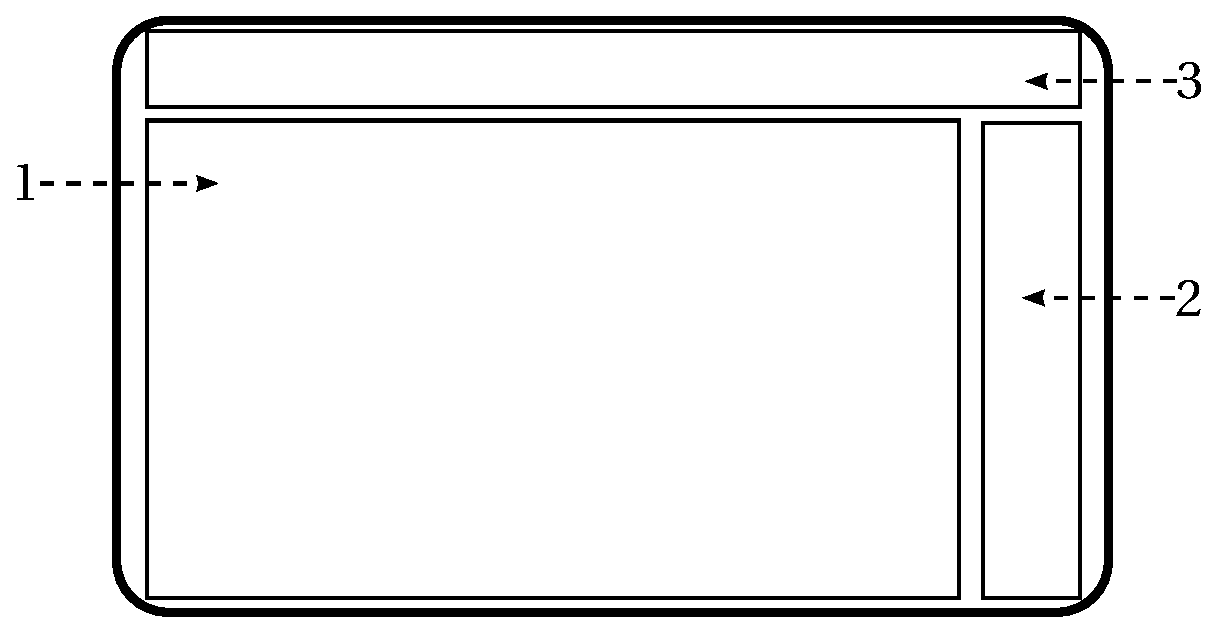
\includegraphics[width=11cm]{./Analyse/Img/14-Editeur_de_niveau.eps}
		\end{center} 
			
	\subsubsection*{Controleur}
		
		Pour finir le contrôleur aura pour but de faire la liaison entre les 
		données du modèle et de la vue.
		Chaque vue possède son controleur.
		Il y a un controleur gobal possédant les controleurs de chaque vue.
			

\subsection{Jeu}
	\subsubsection{Intelligence artificielle}
	
		Comme nous avons vu dans le cahier des charges, nous avons mis en 
		place une intelligence artificielle permettant à un joueur de jouer 
		en solotaire.
	
		Tout d'abord nous avons dû réfléchir à toutes les actions que les 
		\glspl{bots} pourraient effectuer, lors d'une partie.
		
		L'intelligence artificielle dans notre jeu utilise des algorithmes de \gls{recherche_op}.
		
		Pour une meilleure expérience de jeu nous avons séparé l'intelligence artificielle en trois niveaux.
		
		$\,$
		
		\begin{itemize}
		  \item Facile
		  \item Moyenne
		  \item Difficile
		\end{itemize}
		
		$\,$
		
		Nous avons utilisé deux types d'algorithmes de \gls{recherche_op} basés sur le \gls{pathfinding}.
		
		\paragraph{Pathfinding}
		
			Le premier algorithme basé sur le parcours en largeur est utilisé quel que soit
			le niveau de l'intelligence artificelle choisie contrairement au second qui n'est utilisé
			que pour la difficulté moyenne et difficile.
		
		\subparagraph{Parcours en largeur\\}
		
			L'algorithme du parcours en largeur dans notre cas, consiste à partir d'un sommet S,
			lister d'abord tous les voisins de S pour ensuite les explorer un par un.
			Ici nous allons donc regarder toutes les cases autour de nous puis regarder
			tous leurs voisins et cela ainsi de suite jusqu'à trouver un point
			correspondant à nos attentes.
			
			Le contexte est le suivant, un \gls{bot} découvre qu'il est sur la trajectoire
			d'explosion d'une bombe est va donc fuir vers la case sûr la plus proche or
			il n'a aucune idée d'où elle se trouve.
			
			L'image suivante représentera la situation initiale :
			
			\begin{center}
				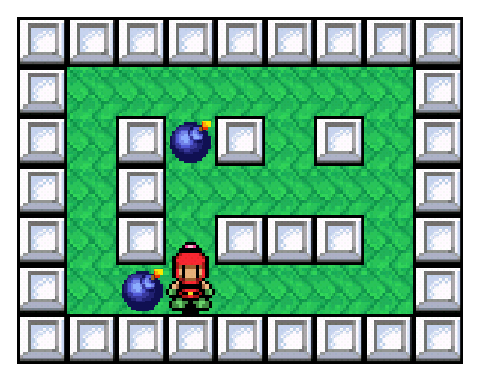
\includegraphics[width=8cm]{./Analyse/Img/largeur_0.eps}
			\end{center}
			
			Comme dit précédemment il n'y a que les murs ou les bombes que l'on ne peut
			pas traverser sinon tous les autres objets ou joueurs sont traversables.
			Nous considerons que les bombes ont ici un champs d'explosion en nombre de
			cases de 5.			
			
			Représentons la carte ci-dessus d'une façon plus parlante en remplacant les
			divers objets mis à par le joueur par des couleurs leur correspondant, à
			savoir :
			
			\begin{center}
				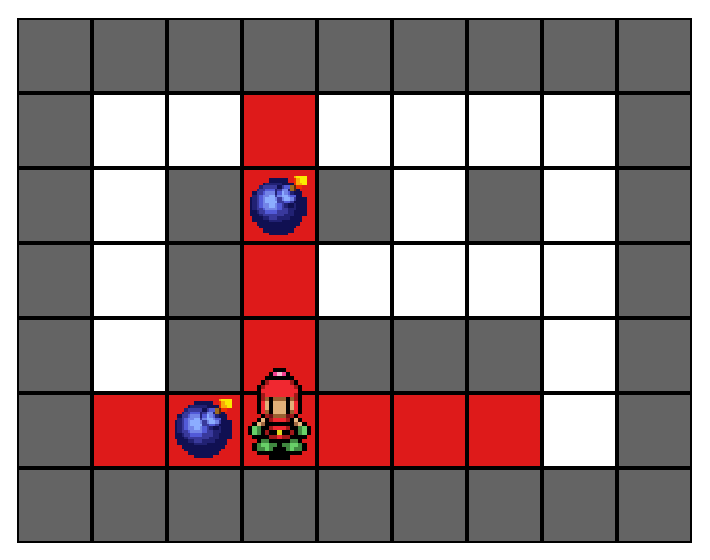
\includegraphics[width=8cm]{./Analyse/Img/largeur_1.eps}
			\end{center}
			
			Mettons nous à present à la place du \gls{bot}.
			
			Nous allons donner un poid aux cases que nous allons parcourir
			correspondant à la distance par rapport à la case initiale, ainsi qu'une
			direction qui correspondra à la direction initiale que le \gls{bot} devra empruter
			pour utiliser ce chemin, c'est à dire par exemple que tout chemin découvert
			dont l'origine est une case à droite de la notre aura comme direction droite.
			
			A partir d'une case donnée, nous ne regarderons que les voisines ayant un poids de 0
			car si leur poids est différent cela voudra dire que nous les avons déjà vu precedemment et bien évidemment,
			nous ignorerons les murs ainsi que les bombes.
			
			Nous avons changé la valeur des cases intraversables pour ne pas confondre avec le poids des cases visitées.			
			
			Appliquons l'algorithme de parcours en largeur aux cases voisines de la notre.
			
			
			\begin{center}
				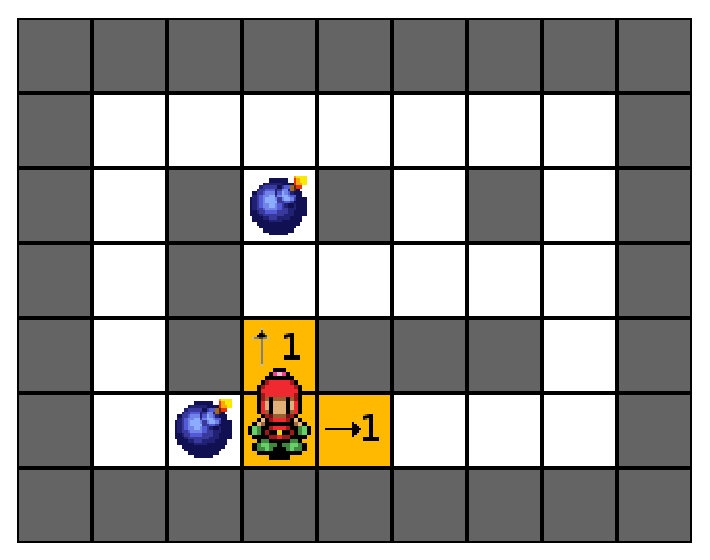
\includegraphics[width=8cm]{./Analyse/Img/largeur_2.eps}
			\end{center}
			
			
			Toutes les cases découvertes étant considérées comme dangereuses (voir le schéma précédent) nous continuons à appliquer l'\gls{algorithme} jusqu'à arriver à notre but.
			
			\begin{center}
				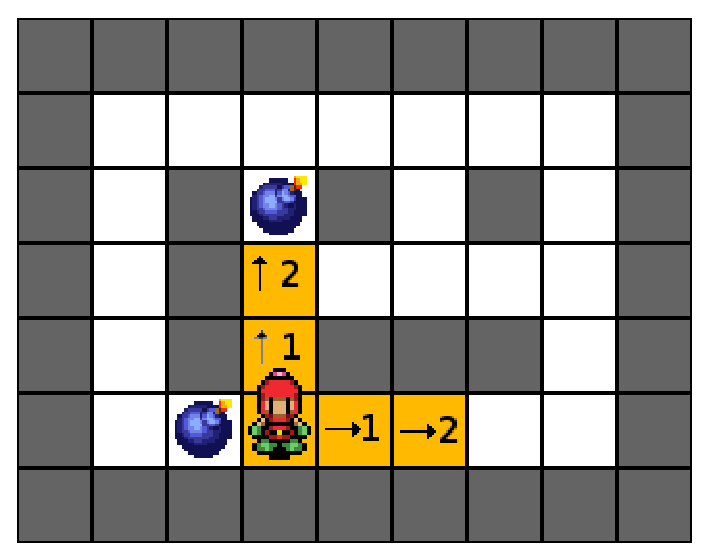
\includegraphics[width=8cm]{./Analyse/Img/largeur_3.eps}
				
				$\,$
				
				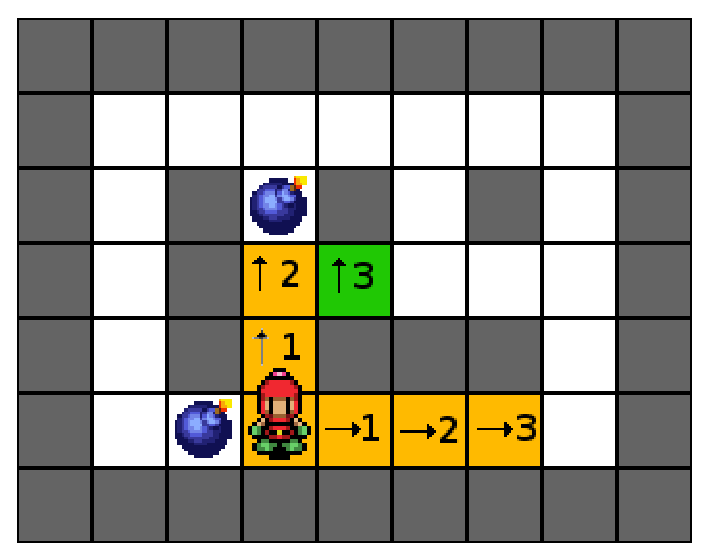
\includegraphics[width=8cm]{./Analyse/Img/largeur_4.eps}
			\end{center}
			
			Ici nous avons découvert une case non dangeureuse en $(13,6)$.
			
			Nous récupérons donc la direction enregistrée dans cette case et bougeons en fonction de celle-ci.
			
			Si plusieurs cases avaient été découvertes le choix aurait été arbitraire car elles auraient toutes été à la même distance.
			
			$\,$
			
		\subparagraph{A*\\}
		
			L'action la plus importante que l'intelligence artificielle doit savoir faire c'est de pouvoir se déplacer librement sur la carte en fonction des différents objets présents sur la carte et des actions effectuées par les autres joueurs.
		
			L'algorithme de recherche A* a pour but de rechercher un chemin
			dans un graphe entre un nœud initial et un nœud final tous deux préalablement
			définis. A* permet de trouver l'un des meilleurs (mais pas forcément le
			meilleur) chemins existant entre un point A et un point B (il retourne le premier chemin trouvé).
			
			La force de cet algorithme est le temps de calcul et l'exactitude des résultats, contrairement à Dijkstra qui lui fournit toujours le meilleur résultat (le plus court chemin entre deux points) mais dans un temps d'exécution beaucoup plus long que l'algorithme de A*.
			
			Sachant qu'il peut y avoir jusqu'à trois \glspl{bot} et que l'intelligence artificielle doit régulièrement recalculer son chemin en fonction des actions effectuées par les autres joueurs, nous avons donc choisi l'algorithme de A*.
		
			Maintenant que l'on sait quel algorithme utiliser pour rechercher un chemin dans un graphe, nous allons voir en détail comment marche l'algorithme de A*.
		
			Pour comprendre comment l'algorithme marche, nous allons nous aider d'un
			dessin représentent une carte avec un point A (départ) affiché en vert, un
			point B (arrivée) en rouge, et où les cases en bleu représentent les murs.
		
			\begin{center}
				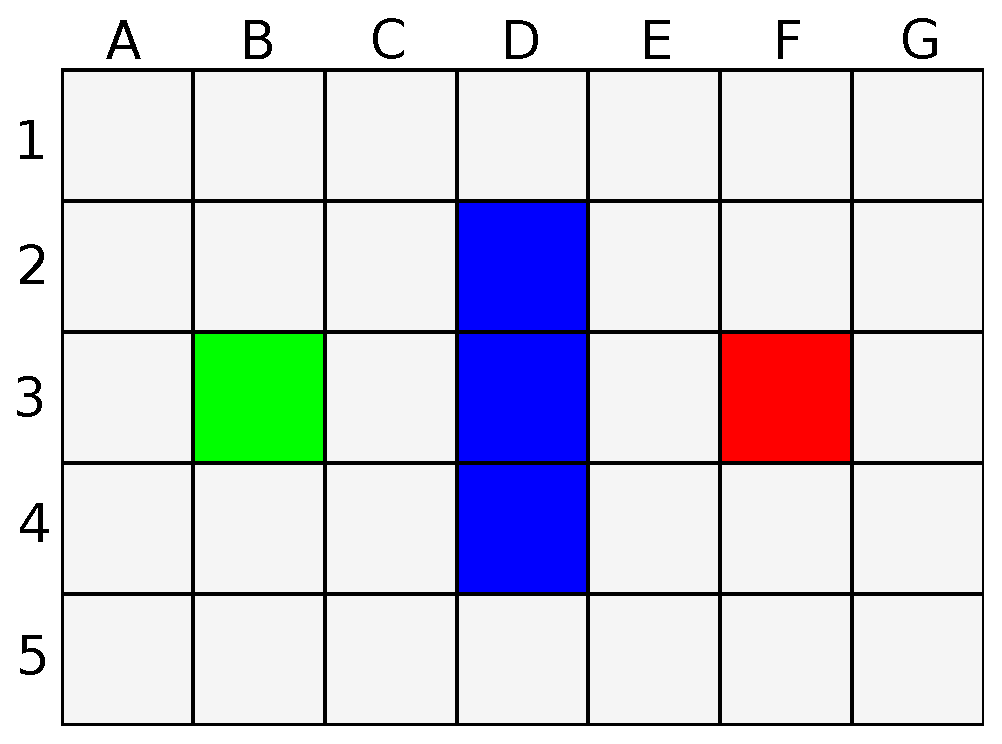
\includegraphics[width=8cm]{./Analyse/Img/Grille.eps}
			\end{center}
		
			La premier chose que l'on peut observer, c'est que la carte est divisée en
			cases. Chaque case de la matrice représente un node qui peut être soit
			traversable, soit non traversable. Dans l'application, il n'y a que les murs
			ou les bombes que l'on ne peut pas traverser sinon tous les autres objets
			ou joueurs sont traversables. Le but de l'algorithme est donc de
			trouver un chemin entre A et B en évitant les murs.
			
		
			Durant le déroulement de l'algorithme, nous avons utilisé deux listes qui contiennent des cases de la carte.
			Il y a une liste dite \og listeOuverte \fg \, et l'autre \og listeFermée \fg.
			La listeOuvrete contient une liste de cases qui pourraient éventuellement faire partie du chemin, mais pas forcément, pour le moment elle sera vide.
			Plus précisément c'est une liste de cases que nous devons vérifier.
			Ensuite, au niveau de la listeFermée, elle contient toutes les cases que nous
			aurons déjà vérifiées, au début de l'excution, elle contient que le point de départ (B3).
			
		
			Commencons les explications du déroulement de l'algorithme.
			Tout d'abord, il faut savoir qu'un joueur peut se déplacer dans toutes les
			directions, donc nous allons ajouter toutes les cases adjacentes à la
			listeOuvert qui sont traversables, il y en a huit (A2, B2, C2, A3, C3, A4, B4, C4).
			
			
			Ce qui nous donne :
		
			\begin{center}
				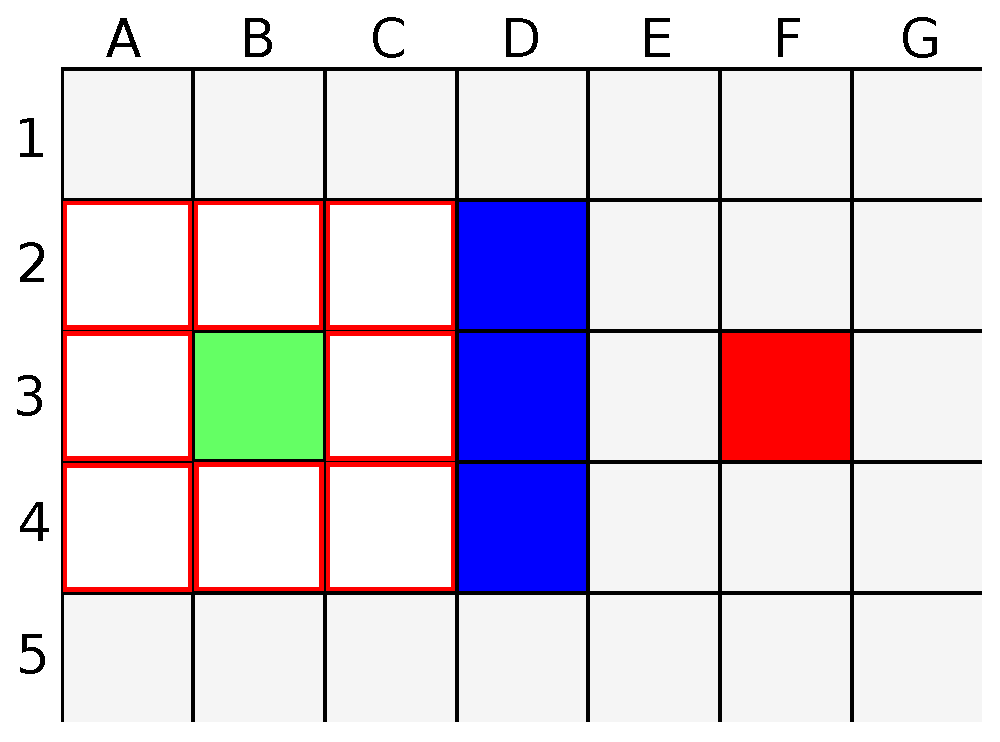
\includegraphics[width=8cm]{./Analyse/Img/Grille2.eps}
			\end{center}
		
			Les carrés avec un contour rouge sont les carrés présents dans la
			listeOuverte et les carrés qui ont une couleur un peu plus foncée que les
			autres sont ceux qui se trouvent dans la listeFermée.
		
			Maintenant pour choisir la case par laquelle on doit passer, nous devons rajouter trois données \og F \fg , \og G \fg \, et \og H \fg:
			\begin{description}
				\item[G : ]{c'est le coût de mouvement pour aller de la case A à une case donnée sur la grille, en suivant le chemin généré jusqu'à cette dernière.}
				\item[H :]{c'est l'heuristique, c'est à dire le coût estimé pour allé du point courant à l'arrivé. Comme nous ne connaissons pas vraiment la distance qu'il nous reste à parcourir, car toutes sortes d'obstacle peuvent se trouver sur notre chemin (objet non traversable). Donc nous allons devoir l'approximer grâce à une fonction, pour la calculer nous avons choisi d'utiliser l'heuristique de Manhattan, qui consiste à compter le nombre de bloc (à vol d'oiseau et sans prendre les diagonales) qui lui reste à parcourir.}
				\item[F :]{c'est G + H}
			\end{description} 
		
			Chaque case de la listeOuverte ou de la listeFermée vont devoir possèder toutes ces données, plus les coordonnées de leur père, c'est à dire les coordonnées de la case qui vient de les ajouter dans la la listeOuverte. Pour calculer G, nous allons assigner un coût de 10 pour chaque déplacement horizontal ou vertical, et un coût de 14 pour un mouvement en diagonale. Nous utilisons ces données car la distance nécessaire pour se déplacer est la racine carrée de 2, ou approximativement 1.41 fois le coût d'un déplacement vertical ou horizontal. Nous utiliserons donc 10 et 14 pour des raisons de simplification. Par conséquent, nous allons multiplier par 10 le coût H pour qu'il soit cohérent par rapport à G.
	
			Donc maintenant, nous devons avoir cette matrice :
			\begin{center}
				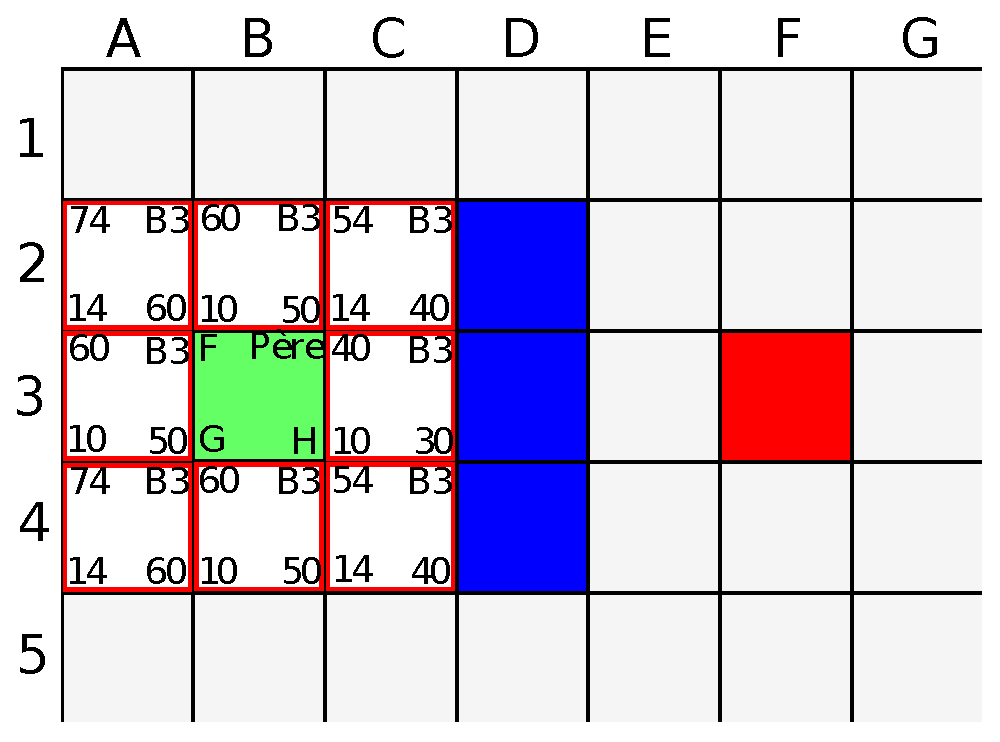
\includegraphics[width=8cm]{./Analyse/Img/Grille3.eps}
			\end{center}
		
			Après avoir ajouté toutes les cases adjacentes à la case courant, il suffit de prendre la case qui a le plus petit coût F et ensuite de la rajouter dans la listeFermée et de la supprimer de la listeOuverte. Nous obtenons donc :
			\begin{center}
				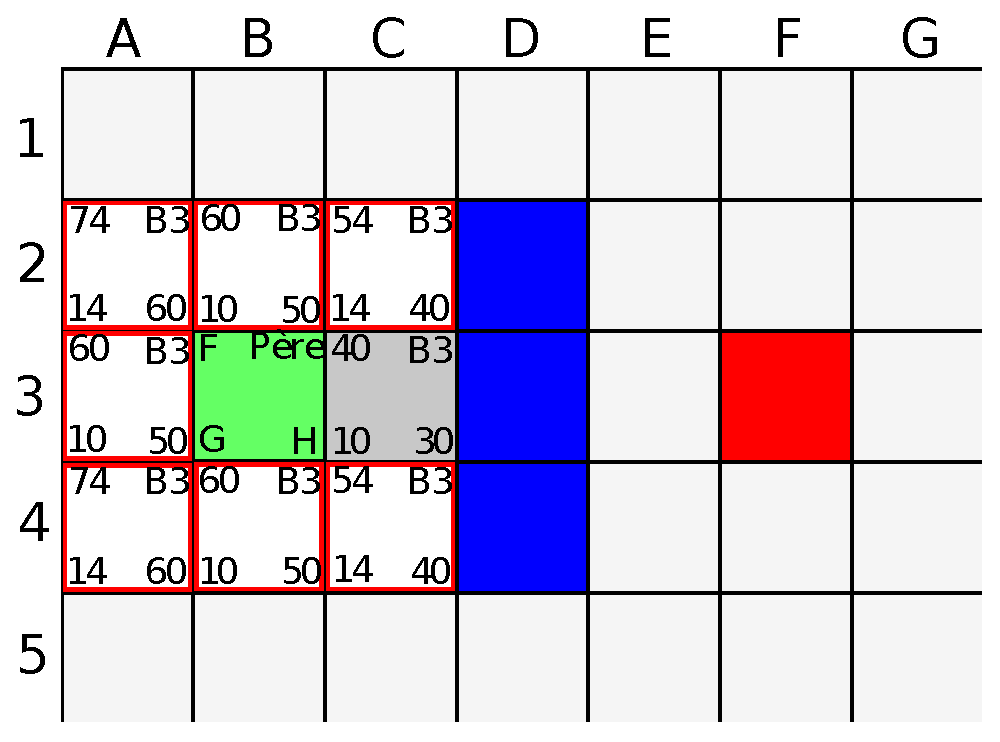
\includegraphics[width=8cm]{./Analyse/Img/Grille4.eps}
			\end{center}
		
			Ensuite on regarde toutes les cases adjacentes à la dernière case ajoutée dans la listeFermée. Si elles se trouvent déjà dans la listeOuverte, on vérifit que leurs coût soient inférieur au coût de la case correspondante déjà dans la listeOuverte, si oui alors on la remplace sinon on ne fait rien.
		
			Pour finir on répète cette opération jusqu'on arrive à la case d'arrivée, nous obtenons ça :
			\begin{center}
				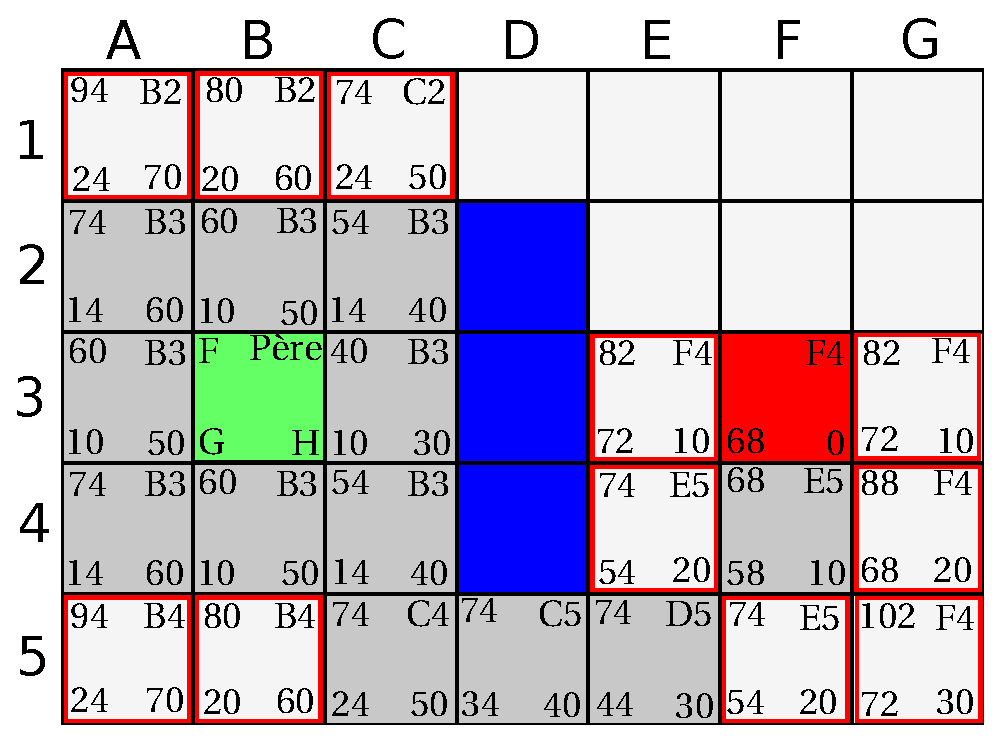
\includegraphics[width=8cm]{./Analyse/Img/Grille5.eps}
			\end{center}
		
			Pour finir, il nous suffit juste de récupérer la case d'arrivée et de regarder son père, puis de repéter cette opération avec la case obtenu jusqu'à arriver à la case de dépard. Grâce à ça nous obtenons cette dernière étape de l'algorithme :
			\begin{center}
				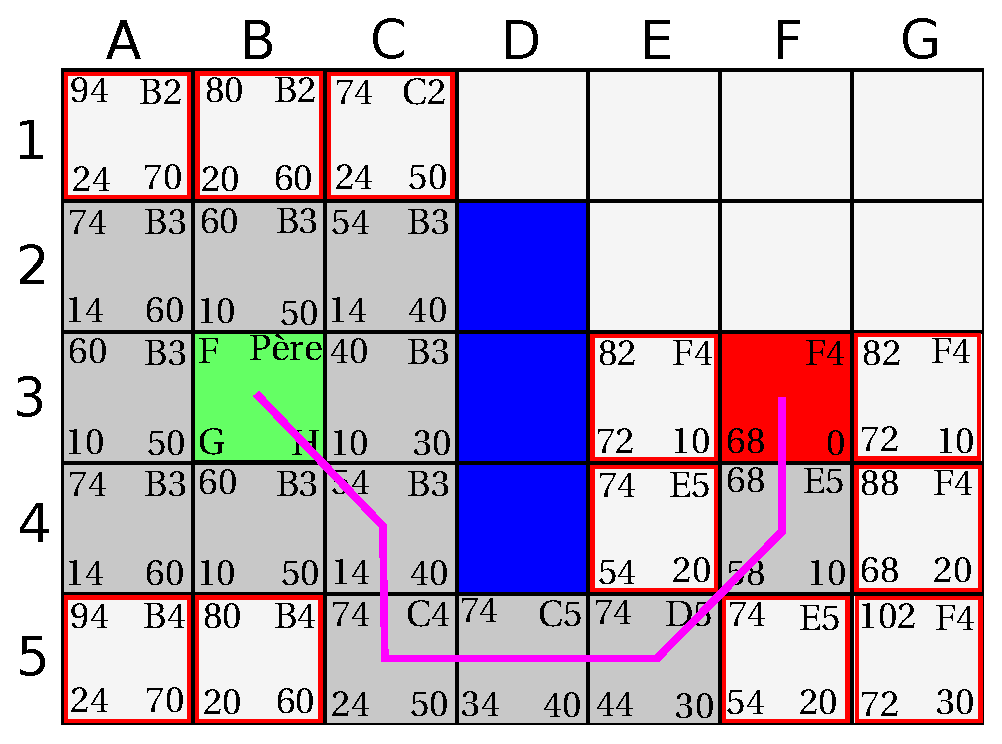
\includegraphics[width=8cm]{./Analyse/Img/Grille6.eps}
			\end{center}
		
			Comme nous pouvons levoir sur le schéma precedent, le chemin qu'a trouvé l'algorithme de A* est le suivant : $ B3 \rightarrow C4 \rightarrow C5 \rightarrow D5 \rightarrow E5 \rightarrow F4 \rightarrow F3 $. L'algorithme aurait pu d'autre chemin équivalent à celui-ci mais le principe de cette algorithme c'est de renvoyer le permier chemin qu'il trouve.
		
	\begin{itemize}
		\item{Diagramme classe}
	\end{itemize}
	
	Comme vue dans le cahier des charges, l'application est divisée en 
	trois grandes parties: le modèle, la vue et le contrôlleur.
	
	\subsubsection{Modèle}
	
		Le modèle constitue la \textit{base} de notre projet.
		C'est sur celui-ci que nous avons construit le reste de l'application.
		Ce dernier se décompose en trois sous-partie: la partie hierarchie des objets, la partie moteur puis la partie éditeur de carte.\\
		
	\paragraph{Hierarchie des objets \\}
	
		Pour concevoir la hierarchie des objets, il a fallu tout d'abord 
		dinstinguer la totalité des objets qui seraient disponibles dans 
		le jeu ainsi que leurs différences et leur point communs.
		
		Pour cela nous avons donc distingué quatre grands types d'objets:
		\begin{itemize}
		  \item Les destructibles
		  \item Les indestructibles
		  \item Les animés
		  \item Les inanimés
		\end{itemize}
		
		En sachant que les objets pouvaient être destructibles-animés, 
		destructible-inanimés, indestructible-animés ou indestructible-inanimés.
		Nous avons choisi que tout objet serait considéré comme un objet animé 
		pour éviter des soucis de modélisation.
		Ainsi les objets possèderont tous une sequence d'animation d'images qui
		 sera dessinée à l'écran.
		Cette dernière sera tournera en boucle dans le cas d'une animation 
		qui se répété et qui comporte plusieurs images, sinon si elle possède 
		simplement qu'une seule image.
		Nous avons ensuite dinstingué une multitude de point communs entre 
		les différents objets dont voici le nom des attributs et leur utilité : 
	
	\begin{description}
		\item [\textit{position}]{indique la position en pixel de l'objet sur l'écran}
		\item [\textit{nom}]{indique le nom de l'objet}
		\item [\textit{hit}]{est à 1 si l'objet ne peut être traversé par un joueur}
		\item [\textit{level}]{est à 0 si l'objet est sur le sol, 1 sinon}
		\item [\textit{fireWall}]{est à 1 si l'objet ne laisse pas passer les flammes des explosions (0,sinon)}
		\item [\textit{damages}]{indique si l'objet peut infliger des dommages}
		\item [\textit{idle}]{est une image qui représente l'objet en son état dit de repos}
		\item [\textit{animates}]{est une table de hachage contenant l'ensemble des images composant la sequence d'animation de l'objet (vide si inanimés)}
		\item [\textit{destroy}]{est une table de hachage contenant l'ensemble des images composant la sequence d'animation de destruction de l'objet (vide si indestructible)}
		\item [\textit{currentFrame}]{permet de connaitre le numéro de l'image courante de la sequence d'animation en cours d'affichage}
	\end{description}

		Nous avons donc décidé de concevoir une classe "Objects" pour modéliser
		 toutes ces propriétés que les objets ont en commun.
		 
		Cette classe sera abstraite car tout objet est destructible ou 
		indestructible et cela sera décris dans des classes plus spécialisés.
	
	 	Ensuite nous avons pensé à créer deux autres classes: "Destructible" 
	 	et "Undestructible" pour les objets destructible et indestructible.
	 	Ces deux classes héritent de "Objects" car elles sont des objets.
	 	
	 	Ce qui différencie ces deux classes est le champ \textit{life} qui 
	 	permet de savoir combien de fois l'objet doit etre touché par une 
	 	bombe avant d'être detruit.
	
		Nous avons ensuite dinstingué deux autres types d"objets encore plus spécifiques :
		Les joueurs et les bombes.
		Ces derniers sont des objets destructibles puisqu'ils ne durent pas 
		toute la partie selon le mode de jeu.
	
		Les bombes possèdent deux nouveaux attributs qui les différentient 
		des autres objets :
		
			\begin{description}
				\item [\textit{type}]{permet de connaitre le type de bombe}
				\item [\textit{owner}]{Joueur qui ayant posé la bombe}
			\end{description}
			
		Quant à la classe joueur celle-ci possède encore d'autres attributs :
		
		\begin{description}
			\item [\textit{color}]{Affiche à l'écran le joueur avec sa bonne couleur}
			\item [\textit{bombsTypes}]{Type de bombe qu'il peut poser}
			\item [\textit{powerExplosion}]{Porté d'explosion de ses bombes}
			\item [\textit{timeExplosion}]{Temps d'explosion de ses bombes}
			\item [\textit{speed}]{Vitesse du joueur}
			\item [\textit{shield}]{Valeur du bouclier}
			\item [\textit{bombNumbers}]{Nombre maximum de bombes que le joueur peut poser}
			\item [\textit{isTouched}]{Permet de savoir si le joueur viens d'être touché}
			\item [\textit{isKilled}]{Permet de savoir si le joueur est mort}
			\item [\textit{isInvincible}]{Permet de savoir si le joueur est invincible}
		\end{description}
	
		Cette hierarchie de classe nous permettra donc de modéliser l'ensemble 
		des objets que le jeu pourra afficher.
	
	
	\paragraph{Moteur\\}
	
		Pour ce qui est du moteur.
		Celui-ci est représenté par une classe "Engine".
		Cette classe va contenir l'ensemble des méthodes qui vont permettrent 
		d'établir les collisions.
		C'est aussi cette classe qui s'occuppe de mettre à jour les bombes 
		ainsi que l'\gls{ia} du jeu.
		
		Une instance d'un moteur est associée à une partie dont le nom de classe est "Game".
		Cette classe "Game" est abstraite et représente une partie avec toutes les options qu'elle contient.
		
		C'est à dire qu'elle possède des attributs permettant de décrire le type de partie,
		un tableau avec chaque joueur de la partie, ainsi que le carte du jeu.
		La classe possède toutes les méthodes d'initialisation, de mise à jour,
		 de dessins et de fin de la partie.
		
		Enfin pour différencier les différents types de parties nous avons utilisé
		 le \gls{pattern} décorateur.
		 Ainsi il y aura deux grands types de parties: les parties solitaires 
		 et les parties multijoueurs.
		 Puis ces parties sont décorés par le type de partie: \gls{survivor} ou \gls{death_match}.
	
		Ensuite pour ce qui est des cartes, une classe abstraite nommé "Map" 
		contient le nom et la taille de la carte ainsi qu'un tableau contenant 
		la position initial de chaque joueur sur la carte.
		
		Puis une classe "GameMap" qui hérite de map permet de dessiner 
		la carte a l'écran lors du jeu.
		Elle se compose d'une image représentant le sol puis d'un tableau 
		d'objets animés qui permet de représenter l'ensemble du reste des objets.
		
		Ensuite nous utilisons un autre type de carte qui va permettre de 
		faciliter les collisions, que ce soit pour un joueur humain ou pour 
		une intelligence artificielle.
		Cette classe est appelé "CollisionMap" et contient une matrice d'objets
		"CollisionCase" ainsi qu'un tableau qui contient l'ensemble des bombes 
		posées sur la carte.
		Les "CollisionCase" sont composées de deux tableaux.
		Chaque valeur d'un des tableaux est associée à une valeur de l'autre tableau.
		Un tableau \textit{types} contient les différents types de danger ou d'objets 
		qui existent sur cette case ainsi qu'un tableau \textit{counters} permettant 
		en fonction de chaque type de compter le nombre de fois que ce danger ou objet 
		est présent sur cette case.
		Par exemple on peut très bien avoir une case qui est dans le champ d'explosion
		de quatres bombes et qui contient un bloc de type destructible.
		
		Ainsi le tableau \textit{type} contiendra deux champs, un pour le 
		type zone dangereuse et un autre pour le type bloc destructible puis 
		le tableau \textit{counters} contiendra donc dans sa case associée à 
		la case zone dangereuse une valeur égale à quatre et et une valeur de
		un pour l'autre.
		
	
	\subsubsection{Vue}
	
		L'interface graphique du jeu est décomposée en trois parties.
		Une partie qui représente le menu d'information de la partie, 
		une autre qui réprésente le menu des actions possibles du joueurs 
		et une dernière qui représente la partie en cours.
		
		Le menu d'information se situe en haut de l'écran.
		Il permet d'afficher le score des joueurs, le temps lors d'une partie 
		death match ainsi que les bonus du joueurs (le nombre de bombes qu'il 
		peut poser, la portée de l'explosion des bombes, la vitesse du joueur 
		et les bonus de vie) et de mettre le jeu en pause.
		
		Le menu d'action se situe à droite de l'écran.
		Il permet à l'utilisateur de poser les bombes grâce à un bouton 
		et aussi de changer de type de bombes grâce à une liste déroulante.
	
		Quant à la partie, elle est affichée au centre de l'écran et prend le 
		maximum de place possible pour que le jeu soit le plus visible.
		Elle permet d'afficher la carte ainsi que les joueurs et les bombes.
		Mais elle sert aussi à écouter les mouvements du doigt de l'utilisateur
		pour modifier les coordonnées du joueur dans le modèle pour pouvoir 
		ensuite rafraichir l'écran et voir le joueur se deplacer.	
	
	
	\subsubsection{Controlleur}
	
		Le controlleur va permettre de faire la liaison entre la vue et le modèle.
		La majorité de ces méthodes sont appelées lorsque l'utilisateur interagit avec la vue.
		Ces méthodes vont par la suite modifier le modèle qui va permettre de mettre à jour la vue.
		Le controlleur est divisé en quatre sous-controlleurs.
		Chacun des trois premiers est respectivement associé à l'une des trois vues cité ci-dessus.
		Puis le quatrième est plus général, il permet de faire la liaison entre les trois autres controlleurs.
		Car en effet chacune des actions effectuées sur l'une des vues peut modifier l'une des deux autres.
	
	\subsubsection{GamePlay}
	
		Nous avons choisi d'établir un gameplay immersif.
		Notre gameplay est divisé en trois parties: les déplacements, la pose des bombes et la gestion des différents types de bombes.
		
		Pour ce qui est des déplacements du joueurs, nous avons décidé que 
		l'utilisateur utiliserait toute la surface de l'écran pour se déplacer.
		Ainsi si il veut se déplacer vers la droite, il fait glisser sont doigt 
		de la gauche vers la droite, puis tant qu'il restera appuyé sur l'écran,
		le joueur continura de se déplacer.
		Cette manière de se déplacer est précise et très intuitive contrairement
		à l'utilisation d'un joystick virtuel ou de l'accéléromètre.
		
		Pour la pause des bombes un simple boutton est mit en évidence en bas à
		 droite de l'écran.
		 Celui-ci est assez gros pour que l'utilisateur n'est pas à appuyer sur
		 une zone trop précise en cas de manipulation rapide.
		
		Puis pour le choix des différentes bombes, une simple liste déroulante 
		est mise en évidence à droite du jeu.\\
		
		\subsubsection{Tile Mapping}

			La gestion des images a été une partie très importante de l'analyse
			car le développement mobile impose plusieurs contraintes, notamment 
			la gestion de la mémoire et la vitesse d'affichage.
			
			Nous nous sommes donc inspirés des premiers jeux consoles comme 
			Super Mario Bros ou Zelda qui ont été développés sur les premières 
			consoles comme la \gls{nes} ou la \gls{game_boy}.
			Nous avons donc conçu le moteur du jeu selon le principe du \gls{tile_mapping} 
			pour minimiser l'utilisation des ressources des téléphones.
		
			Le principe du Tile Mapping est d'utiliser des petites images que nous appelerons \textit{tiles}.
			Ces tiles sont toutes contenues dans une image.
			Ensuite une matrice de nombre entier est utilisé pour représenter l'environnement du jeu.
			Chaque nombre entier représente un tile.
			Puis grâce à cette association, la carte sera dessiné à l'écran selon la matrice.
			Voici un exemple :
		
			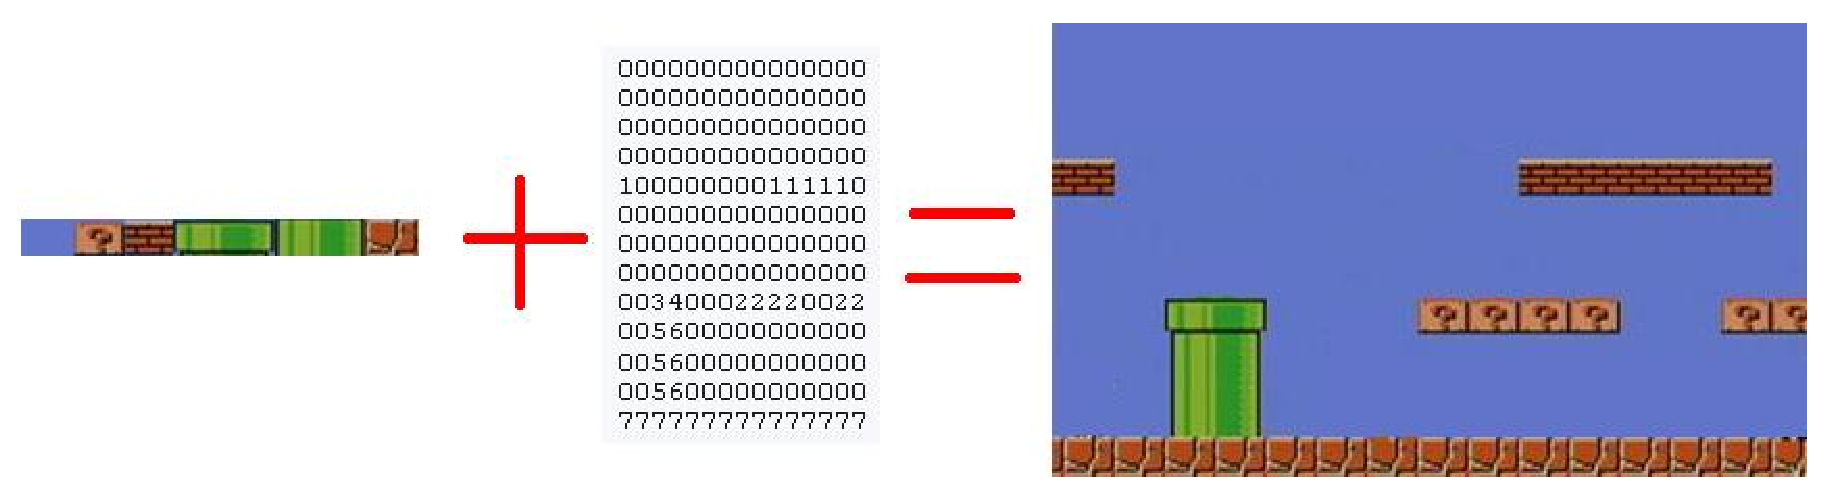
\includegraphics[width=15cm]{./Analyse/Img/tileMapping.eps}
		
			Pour pouvoir animer certains de ces objets nous avons utilisé des sprites.
			Les sprites contrairement aux tile sont un ensemble d'images représentant
			une animation.
		
			Nous avons donc repris ce principe et nous l'avons amélioré.
			En effet grâce à la programmation objet, les entiers sont réprésenté directement par des objets
			contenant les tiles/sprites qui les représentent.
			
			Ainsi, nous stockons dans une matrice tous les objets inanimés
			(les objets dont le tile restera le meme tout le long de la partie)
			et nous parcourons cette matrice pour dessiner chaque objet à sa 
			position pour obtenir une nouvelle image au format png.
			A chaque rafraichissement de l'écran, seule la nouvelle image est dessinée 
			et non pas chaque tile.
			Cette méthode permet d'éviter un parcours intempestif de la matrice.
			
			Ensuite pour le reste des objets dit animés (repésentés par des sprites)
			nous avons décidé de les stocker dans une table de hachage dont la 
			clé est la position de l'objet (pour y accéder plus rapidement).
			Lors du rafraichissement de l'écran on parcourra entierement la 
			table de hachage et l'on dessinera l'image courante de la sequence 
			d'animation de chaque objet.
		
		\subsubsection{La gestion des images et du son}
		
			Chaque image et chaque son dont est composé le jeu sont chargés au lancement de l'application.
 			
 			Afin de pouvoir ajouter facilement un objet et le modifier sans avoir à toucher au code
 			source, nous avons décidé d'opter pour les stocker sur des fichiers au format \gls{xml}
 			Les fichiers \gls{xml} ressemblent tous plus au moins a ce genre d'arborescence: 
		
		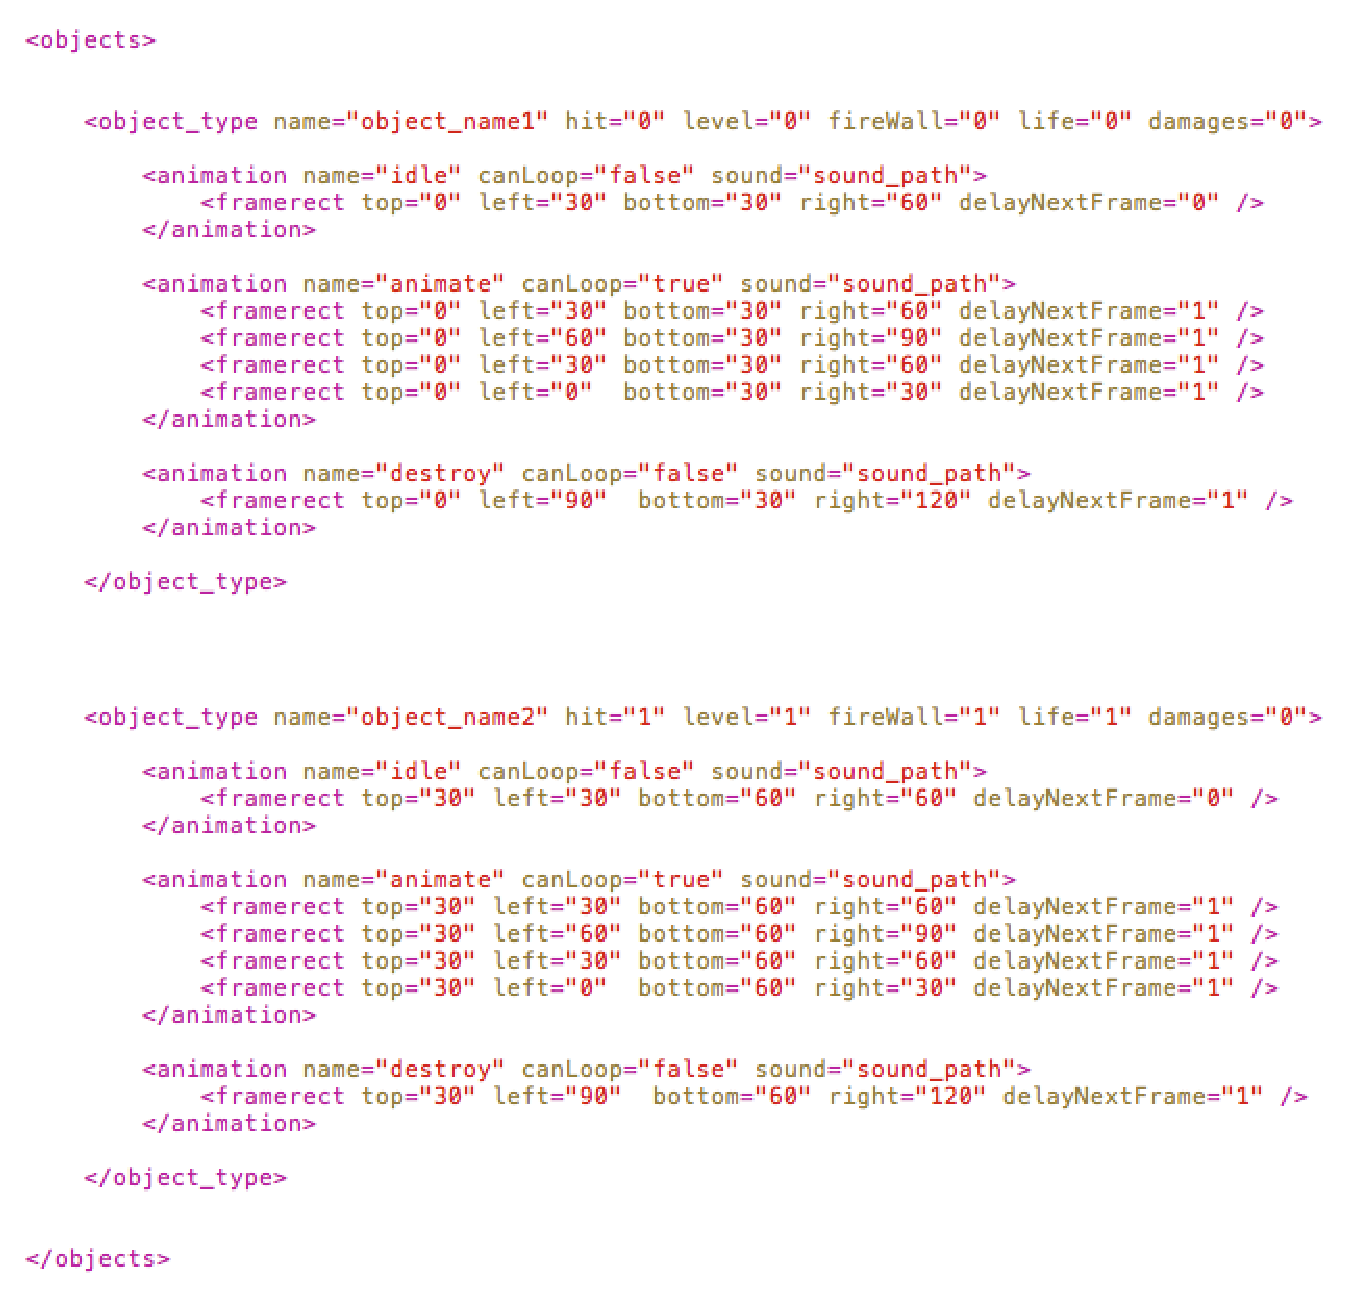
\includegraphics[width=15cm]{./Analyse/Img/exampleXmlBomberklob.eps}
		
			Chaque fichier \gls{xml} commence par une balise racine permettant 
			de lister les objets qu'elle contient (\textit{<objects>}).
			Ensuite chaque objet est décris par une balise  qui contient le type,
			le nom de l'objet ainsi que l'ensemble de ses propriétés.
			
			La propriété \textit{hit} est à 1 si l'objet n'est pas traversable par un joueur (0, sinon), 
			le champ \textit{level} est à 1 si l'objet se trouve au premier niveau de la carte (0,sinon), 
			le champ \textit{fireWall} est à 1 si l'objet ne laisse pas passer les flammes des explosions, 
			le champ \textit{life} indique le nombre de fois que l'objet doit etre touché
			et enfin le champ \textit{damages} indique si l'objet peut infliger des domages.
			
			Par exemple \textit{<destructible name="herb" hit="1" level="1" fireWall="1" life="1" damages="0">} 
			décris un objet de type \textit{destructible}, qui n'est pas traversable, se trouvant au niveau
			1 sur la carte, ne laissant pas passer les flammes des bombes, possedant une vie, 
			n'infligeant pas de dommage et dont le nom est \textit{herb}.
			
			Ensuite chaque objet possède au plus trois balises animations (sauf pour les joueurs).
			Tout objet possède au moins la premiere balise: 
			<animation name="idle" canLoop="false" sound="sound\_path"> 
			qui est celle dont le nom est \textit{idle}.
			
			Elle représente l'image standard de l'objet.
			Par exemple pour un objet bombe, ce sera l'image qui sera affichée dans la liste des bombes 
			pour pouvoir selectionner ses bombes.
			Le champs \textit{canLoop} permet de savoir si l'animation doit être répétée en boucle 
			et le champ \textit{sound} contient le chemin d'accès au fichier de son de l'animation 
			si elle en possede un.
			
			Il y a ensuite la balise mais dont le nom est \textit{animate}, celle-ci contiendra *
			toutes les sequences d'images d'un objet qui est animés.
			La dernière est celle dont le nom est \textit{destroy} et qui contiendra 
			l'ensemble des images composant la sequences d'animation de destruction de l'objet.
			Enfin chaque balise de type animation contient des balises de type \textit{framerect}.
			Ces balises permettent de donner la position de chaque image de la séquence d'animation
			dans la bitmap globale ainsi que le delai de rafraichissement entre chaque image.
			Par exemple \textit{<framerect top="60" left="30" bottom="90" right="60" delayNextFrame="1" />}
			représente une image dont le bord du haut est situé à 30pixels, le bord du bas à 90pixels, 
			le bord de gauche à 30pixels et le bord de droite à 60pixels en partant du coin en haut à 
			gauche de l'image globale.
			Puis pour le champ \textit{delayNextFrame} celui-ci informe que l'image suivante sera déclenchée 
			apres un delay de 1s.\\
		
			Grâce à cette modélisation, l'application va parcourir au démarrage l'ensemble des fichiers 
			XML et va créer une table de hachage pour chaque ensemble d'objet du fichier.
			Lors de ce parcours, l'application va instancier chaque objet avec toutes propriétés 
			que lui indique le document XML, ainsi que ses sequences d'animations.
			Ensuite lorsqu'un objet devra être utilisé dans le jeu, il suffira d'utiliser 
			une copie de l'objet déja chargé en mémoire pour éviter d'avoir à reparcourir le fichier.


\subsection{Réseau}
		
	\paragraph{Serveur\\}
			
		Il a été fixé dans le cahier des charges que notre serveur devrait pouvoir
		effectuer plusieurs tâches particulières séparées. Nous avons donc décidé de
		les compartimenter en classes.
		
		Notre serveur est crée sur une base de servlet. Ce fût ici
		aussi un point nouveau pour nous, réiterant les phases d'analyse, de
		découverte, de test et de mise en place. Le fonctionnement est basé sur les
		échanges de requêtes type HTTP, où à chaque demande correspond une réponse. 
		
		Une servlet est une classe Java qui permet de créer dynamiquement des données
		au sein d'un serveur HTTP. Une servlet s'exécute dynamiquement sur le serveur
		web et permet l'extension des fonctions de ce dernier, typiquement : accès à
		des bases de données.
			
		Les six éléments situés sur la partie haute du schéma
		ci-dessous(respectivement ServletInscription, ServletConnection,
		ServletGamesList, ServletCreateGame, ServletConnectionGame et
		ServletManageGame), représentent les différentes tâches qu'un utilisateur
		puisse demander au serveur. Elles sont reliées à une classe nommée
		ContextListener, qui leur permettra d'accéder aux mêmes données sans qu'il y
		ait de conflit. La partie basse représente les objets qui seront utilisés 
		pour les parties en multijoueur. 
		Bien évidemment ces objets sont très proches de ceux utilisés dans les parties
		locales(Schéma 3.3).
		
		
		Comme il a été dit précédement, notre serveur est accessible via des requêtes
		HTTP contactant des servlets. Ces servlets sont stockées dans un serveur
		d'application nommé Apache Tomcat. Il s'agit d'un conteneur libre de
		servlets Java 2 Enterprise Edition, mais il fait aussi office de serveur
		Web.\\
		Un scénario probable serait qu'un utilisateur désire jouer
		en ligne contre de vrais joueurs. 
		Il passera par l'inscription et créera son compte sur le
		serveur(Inscription). Une fois cette étape obligatoire faite, il choisira
		entre rejoindre une partie en ligne en cour(ConnectionGame), ou en créer un nouvelle(CreateGame).
		Dès lors qu'il accèdera à une partie en
		ligne, un contact régulier avec le serveur sera obligatoire afin de réaliser
		les interactions entre les joueurs(ManageGame). Tout ceci se
		réalisera dans une durée infime afin de ne pas pénaliser les joueurs.	
		
		\begin{figure}
			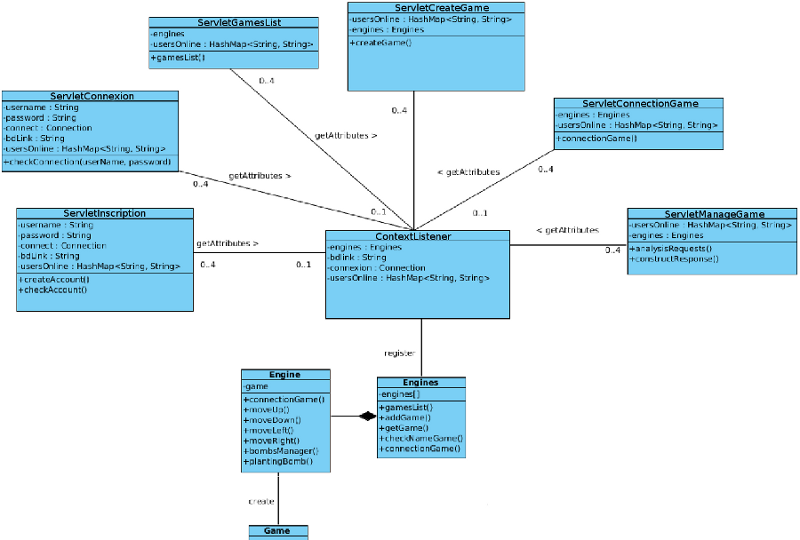
\includegraphics[scale = 0.5]{Analyse/Img/serveur.eps}
			 \caption {Serveur}
		\end{figure}
		
		\newpage
		
		
	\paragraph{JSON\\}	
	
		Soucieux des performances et de la rapidité des échanges entre applications et
		serveur, nous avons mis en place un protocole de communication client/serveur
		où les messages transitant sont des flux \gls{json}. 	
		Contrairement au \gls{xml} qui peut représenter des données orientées document,
		\gls{json} se focalise sur la description d’objets.
		Un autre avantage reconnu de \gls{json} par rapport à \gls{xml} est qu’il est nettement
		moins verbeux que ce dernier.
		Quoi qu’il en soit \gls{json} reconnait la philosophie des services web exposant
		une interface d’échange : il s’agit
		d’envoyer et de recevoir des informations dans un format facilement manipulable par
		le protocole de transport \gls{http}.
		
		
		Voilà pourquoi le \gls{json} semblait être un format de données d'échanges optimal
		pour véhiculer le plus d'informations avec une taille moindre. Il est aussi en
		adéquation avec notre politique d'utilisation web pour un serveur.
		De plus étant beaucoup utilisé, nos deux
		langages mettent à disposition des outils de sérialisation de leurs objets en \gls{json}
		
		Ci-dessous un exemple concret de notre protocole de communication \gls{json} entre
		serveur et application cliente.
		
			
		\begin{verbatim}
			ServletInscription
				Player => Serveur
				{["username","password"]}
				
				Serveur => Player
				{"OK"} ou {"BU"}
				
			ServletConnexion 	
				Player => Serveur
				{["username","password"]}
				
				Serveur => Player
				{"OK"} ou {"BU"}
				
			ServletGameList
				Player => Serveur
				{"userKey"}
			
				Serveur => Player
				{[{"class":"Game","map":"mapName","name":"gameName",
				 "playerNumberConnected":nbConnected,"type":"gameType"},{..},{..}]}
				 
			ServletCreateGame:
				Player => Server:
					{"userKey": <userKey>, 
					"game": {"name":<name>, "type":<type>, "map":<map>, "ennemiesNumber": <ennemiesNumber>}}
					
				Server => Player:
					{"OK"} ou {"errorType"}
				 
			ServletConnectionGame:
				Player => Server:
					{["userKey", "gameName"]}
					
				Server => Player:
					{[<1/2/3/4>, "play<true/false>", "map", "time<mm:ss>"]} 
					ou 
					{"errorType"}
					
			ServletManageGame:
				Player => Server: 
					{"userKey", "gameName", "action"}	
					
				Server => Players: (Player, bombs, blocs, score, time)
					{[
					 [ ["x", "y", "direction", "dead <true/false>"],[...] ],
					 [ ["x", "y", "type", "explode <true/false>" ], [...] ],
					 [ ["position": {"x", "y"}, "bonus": <bonus>], [..] ],
					 [1,2,3,4],
					 "time <mm:ss>"]} 
					 ou 
					{"errorType"}
				 
				 
		\end{verbatim}	
		
	

	\subsubsection{Schéma de fonctionnement }
		
		\begin{center}
			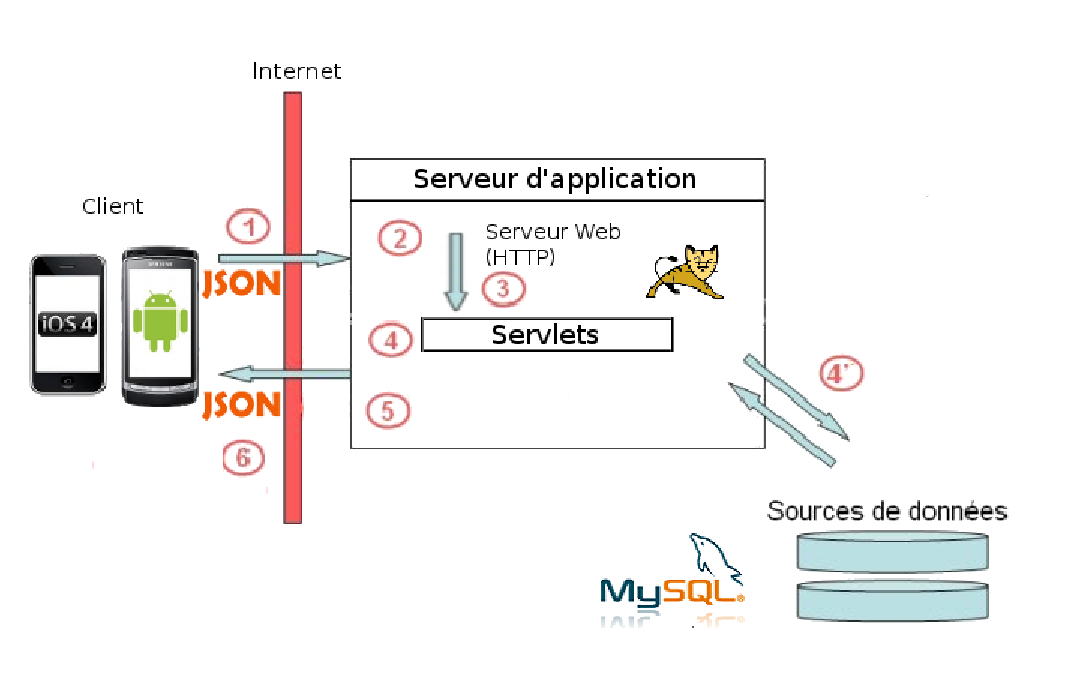
\includegraphics[width=16cm]{Analyse/Img/4.eps}
		\end{center}
		
		\begin{enumerate}

			\item 
					Le client émet une requête pour demander une
					ressource au serveur. Par exemple la création de son compte multijoueur,
					qui pourrait se situer \url{http://Bomberklob.com/inscription}
			\item
					Côté serveur, c'est le serveur web qui traite les
					requêtes HTTP entrantes. Il traite donc toutes les requêtes, qu'elles
					demandent une ressource statique ou dynamique. Seulement, un serveur HTTP
					ne sait répondre qu'aux requêtes visant des ressources statiques.

			\item 
					Ainsi, si le serveur HTTP s'aperçoit que la requête reçue est destinée
					au serveur d'applications, il la lui transmet. Les deux serveurs sont
					reliés par un canal, nommé connecteur.
		
			\item
					Le serveur d'applications (dans notre cas Tomcat) reçoit la requête à
					son tour. Lui est en mesure de la traiter. Il exécute donc la servlet
					correspondante à la requête, en fonction de l'URL, en récupérant les
					valeurs dans le flux JSON entrant. Cette opération est effectuée à partir
					de la configuration du serveur, grâce un fichier web.xml faisant le mapping
					entre URL et servlet associée.
		
					La servlet est donc invoquée, et le serveur lui fournit notamment deux
					objets Java exploitables: un représentant la requête, l'autre représentant
					la réponse. La servlet execute sa fonction et génère la réponse à la
					demande, sous forme de flux JSON. Cela peut passer par la consultation de
					sources de données, comme des bases de données (4' sur le schéma).		
		
		\end{enumerate}
		
	\paragraph{Base de données\\}
		Afin de pouvoir conserver les utilisateurs en ligne ainsi que leurs infos
		personnels et permettre une authentification, nous avons dû établir une
		base de données sur le serveur. Cette dernière à été pensé comme demandé pour 
		l'enregistrement de comptes. Une unique table nommée Users remplie donc cette
		fonction. Le serveur devra pouvoir y accéder en écriture(inscription) comme
		en lecture(connexion).
			Aléatoire
		Elle ne comportera que deux champs, userName et password. Dès lors que
		l'utilisateur désirera créer un compte multijoueur, il renseignera dans
		l'application son userName souhaité ainsi que son mot de passe. 
		Ce couple sera 	alors envoyé au serveur qui vérifiera dans cette base de
		données, que le userName(unique) n'est pas déjà utilisé. Auquel cas un nouveau n-uplet sera
		inséré et permettra l'authentification de l'utilisateur par la suite. Les mots
		de passe seront bien évidement crypté pour des raisons de sécurité.
			

		\newpage
		
	